%  LaTeX support: latex@mdpi.com 
%  For support, please attach all files needed for compiling as well as the log file, and specify your operating system, LaTeX version, and LaTeX editor.

%=================================================================
\documentclass[foods,article,submit,moreauthors,pdftex]{Definitions/mdpi} 

% For posting an early version of this manuscript as a preprint, you may use "preprints" as the journal and change "submit" to "accept". The document class line would be, e.g., \documentclass[preprints,article,accept,moreauthors,pdftex]{mdpi}. This is especially recommended for submission to arXiv, where line numbers should be removed before posting. For preprints.org, the editorial staff will make this change immediately prior to posting.

%--------------------
% Class Options:
%--------------------
%----------
% journal
%----------
% Choose between the following MDPI journals:
% acoustics, actuators, addictions, admsci, adolescents, aerospace, agriculture, agriengineering, agronomy, ai, algorithms, allergies, analytica, animals, antibiotics, antibodies, antioxidants, appliedchem, applmech, applmicrobiol, applnano, applsci, arts, asi, atmosphere, atoms, audiolres, automation, axioms, batteries, bdcc, behavsci, beverages, biochem, bioengineering, biologics, biology, biomechanics, biomedicines, biomedinformatics, biomimetics, biomolecules, biophysica, biosensors, biotech, birds, bloods, brainsci, buildings, businesses, cancers, carbon, cardiogenetics, catalysts, cells, ceramics, challenges, chemengineering, chemistry, chemosensors, chemproc, children, civileng, cleantechnol, climate, clinpract, clockssleep, cmd, coatings, colloids, compounds, computation, computers, condensedmatter, conservation, constrmater, cosmetics, crops, cryptography, crystals, curroncol, cyber, dairy, data, dentistry, dermato, dermatopathology, designs, diabetology, diagnostics, digital, disabilities, diseases, diversity, dna, drones, dynamics, earth, ebj, ecologies, econometrics, economies, education, ejihpe, electricity, electrochem, electronicmat, electronics, encyclopedia, endocrines, energies, eng, engproc, entropy, environments, environsciproc, epidemiologia, epigenomes, fermentation, fibers, fire, fishes, fluids, foods, forecasting, forensicsci, forests, fractalfract, fuels, futureinternet, futuretransp, futurepharmacol, futurephys, galaxies, games, gases, gastroent, gastrointestdisord, gels, genealogy, genes, geographies, geohazards, geomatics, geosciences, geotechnics, geriatrics, hazardousmatters, healthcare, hearts, hemato, heritage, highthroughput, histories, horticulturae, humanities, hydrogen, hydrology, hygiene, idr, ijerph, ijfs, ijgi, ijms, ijns, ijtm, ijtpp, immuno, informatics, information, infrastructures, inorganics, insects, instruments, inventions, iot, j, jcdd, jcm, jcp, jcs, jdb, jfb, jfmk, jimaging, jintelligence, jlpea, jmmp, jmp, jmse, jne, jnt, jof, joitmc, jor, journalmedia, jox, jpm, jrfm, jsan, jtaer, jzbg, kidney, land, languages, laws, life, liquids, literature, livers, logistics, lubricants, machines, macromol, magnetism, magnetochemistry, make, marinedrugs, materials, materproc, mathematics, mca, measurements, medicina, medicines, medsci, membranes, metabolites, metals, metrology, micro, microarrays, microbiolres, micromachines, microorganisms, minerals, mining, modelling, molbank, molecules, mps, mti, nanoenergyadv, nanomanufacturing, nanomaterials, ncrna, network, neuroglia, neurolint, neurosci, nitrogen, notspecified, nri, nursrep, nutrients, obesities, oceans, ohbm, onco, oncopathology, optics, oral, organics, osteology, oxygen, parasites, parasitologia, particles, pathogens, pathophysiology, pediatrrep, pharmaceuticals, pharmaceutics, pharmacy, philosophies, photochem, photonics, physchem, physics, physiolsci, plants, plasma, pollutants, polymers, polysaccharides, proceedings, processes, prosthesis, proteomes, psych, psychiatryint, publications, quantumrep, quaternary, qubs, radiation, reactions, recycling, regeneration, religions, remotesensing, reports, reprodmed, resources, risks, robotics, safety, sci, scipharm, sensors, separations, sexes, signals, sinusitis, smartcities, sna, societies, socsci, soilsystems, solids, sports, standards, stats, stresses, surfaces, surgeries, suschem, sustainability, symmetry, systems, taxonomy, technologies, telecom, textiles, thermo, tourismhosp, toxics, toxins, transplantology, traumas, tropicalmed, universe, urbansci, uro, vaccines, vehicles, vetsci, vibration, viruses, vision, water, wevj, women, world 

%---------
% article
%---------
% The default type of manuscript is "article", but can be replaced by: 
% abstract, addendum, article, book, bookreview, briefreport, casereport, comment, commentary, communication, conferenceproceedings, correction, conferencereport, entry, expressionofconcern, extendedabstract, datadescriptor, editorial, essay, erratum, hypothesis, interestingimage, obituary, opinion, projectreport, reply, retraction, review, perspective, protocol, shortnote, studyprotocol, systematicreview, supfile, technicalnote, viewpoint, guidelines, registeredreport, tutorial
% supfile = supplementary materials

%----------
% submit
%----------
% The class option "submit" will be changed to "accept" by the Editorial Office when the paper is accepted. This will only make changes to the frontpage (e.g., the logo of the journal will get visible), the headings, and the copyright information. Also, line numbering will be removed. Journal info and pagination for accepted papers will also be assigned by the Editorial Office.

%------------------
% moreauthors
%------------------
% If there is only one author the class option oneauthor should be used. Otherwise use the class option moreauthors.

%---------
% pdftex
%---------
% The option pdftex is for use with pdfLaTeX. If eps figures are used, remove the option pdftex and use LaTeX and dvi2pdf.

%=================================================================
% MDPI internal commands
\firstpage{1} 
\makeatletter 
\setcounter{page}{\@firstpage} 
\makeatother
\pubvolume{1}
\issuenum{1}
\articlenumber{0}
\pubyear{2021}
\copyrightyear{2020}
%\externaleditor{Academic Editor: Firstname Lastname} % For journal Automation, please change Academic Editor to "Communicated by"
\datereceived{} 
\dateaccepted{} 
\datepublished{} 
\hreflink{https://doi.org/} % If needed use \linebreak
%------------------------------------------------------------------
% The following line should be uncommented if the LaTeX file is uploaded to arXiv.org
%\pdfoutput=1

%=================================================================
% Add packages and commands here. The following packages are loaded in our class file: fontenc, inputenc, calc, indentfirst, fancyhdr, graphicx, epstopdf, lastpage, ifthen, lineno, float, amsmath, setspace, enumitem, mathpazo, booktabs, titlesec, etoolbox, tabto, xcolor, soul, multirow, microtype, tikz, totcount, changepage, paracol, attrib, upgreek, cleveref, amsthm, hyphenat, natbib, hyperref, footmisc, url, geometry, newfloat, caption

\setlength{\headheight}{22pt}
\usepackage{times}
\usepackage{amssymb}
\newcommand{\ignore}[1]{}
\usepackage{tikz}
\usetikzlibrary {arrows}
\usetikzlibrary{arrows.meta}
\usepackage[export]{adjustbox}
% \usepackage{caption}
\usepackage{graphicx}
\usetikzlibrary{fit}
\usepackage{textgreek}
% \usepackage{gensymb}
\usepackage[hang]{footmisc}
% \usepackage{cite}
\usepackage{mathrsfs,amsmath}
\usepackage{pifont}
\usepackage{booktabs}
\usepackage{graphicx}
\usepackage{array}
\aboverulesep=0ex
\belowrulesep=0ex
\usepackage{cleveref}

\usepackage{subcaption}
% \captionsetup[subfigure]{justification=centering,labelfont=normal}
\renewcommand{\thesubfigure}{(\alph{subfigure})}
% \captionsetup[sub]{labelformat=simple}
%Notes
\usepackage[textwidth=11mm]{todonotes}
\setlength{\marginparwidth}{2cm}
\newcommand{\mymark}[1]{\todo[color=green!20!white,inline,size=\small, author=O.]{#1}}
\newcommand{\mynote}[1]{\todo[color=green!20!white,size=\small]{zor.: #1}}
\setuptodonotes{inline}
% \hypersetup{breaklinks=true,
%             unicode=true,}




%=================================================================
%% Please use the following mathematics environments: Theorem, Lemma, Corollary, Proposition, Characterization, Property, Problem, Example, ExamplesandDefinitions, Hypothesis, Remark, Definition, Notation, Assumption
%% For proofs, please use the proof environment (the amsthm package is loaded by the MDPI class).

%=================================================================
% Full title of the paper (Capitalized)
%\Title{Label-free mapping and dynamic analysis of food industry biofilms and planktonic bacteria using Fourier-transform infrared spectroscopy techniques}

%\Title{Label-free mapping and dynamic analysis of food industry biofilms and planktonic bacteria on steel  using Fourier-transform infrared spectroscopy techniques}

%\Title{Biofilms and planktonic bacteria: a closer look on the applicability of Fourier-transform infrared spectroscopy techniques}

% MDPI internal command: Title for citation in the left column
\TitleCitation{Label-free mapping and dynamic analysis of food industry biofilms using Fourier-transform infrared spectroscopic techniques}
\Title{Observing biofilm and planctonic bacteria on stainless steel in food industry by FTIR spectroscopic techniques re-visited}


% Author Orchid ID: enter ID or remove command
\newcommand{\orcidauthorA}{0000-0000-0000-000X} % Add \orcidA{} behind the author's name
%\newcommand{\orcidauthorB}{0000-0000-0000-000X} % Add \orcidB{} behind the author's name
\newcommand{\orcidauthorC}{0000-0001-9933-0330} % Add \orcidC{} behind the author's name

% Authors, for the paper (add full first names)
\Author{Elisabeth Leiss-Holzinger $^{1\ignore{,\dagger,\ddagger}}$\orcidA{}, Eva M. Wagner $^{2\ignore{,\ddagger}}$,  Robert Zimmerleiter$^{1\ignore{,\dagger,\ddagger}}$\orcidC{}, Ivan Zorin$^{1\ignore{,\dagger,\ddagger}}$, Kathrin Rychli$^{2\ignore{,\ddagger}}$  and Markus Brandstetter $^{1,}$*}

% MDPI internal command: Authors, for metadata in PDF
\AuthorNames{Elisabeth Leiss-Holzinger, Eva Maria Wagner , Kathrin Rychli and Markus Brandstetter}

% MDPI internal command: Authors, for citation in the left column
\AuthorCitation{Leiss-Holzinger, E.; M. Wagner,  E.; Brandstetter, M.}
% If this is a Chicago style journal: Lastname, Firstname, Firstname Lastname, and Firstname Lastname.

% Affiliations / Addresses (Add [1] after \address if there is only one affiliation.)
\address{%
$^{1}$ \quad Research Center for Non-Destructive Testing, Science Park 2, Altenberger Str.69, 4040 Linz, Austria\\
$^{2}$ \quad FFoQSI GmbH – Austrian Competence Centre for Feed and Food Quality, Safety and Innovation, 3430 Tulln, Austria}

% Contact information of the corresponding author
\corres{Correspondence: \href{mailto:markus.brandstetter@recendt.at}{markus.brandstetter@recendt.at}}

% Current address and/or shared authorship
% \firstnote{Current address: Affiliation 3} 
% \secondnote{These authors contributed equally to this work.}
% The commands \thirdnote{} till \eighthnote{} are available for further notes

%\simplesumm{} % Simple summary

%\conference{} % An extended version of a conference paper

% Abstract (Do not insert blank lines, i.e. \\) 
\abstract{Biofilms are communities of bacteria shielded by a self-produced matrix. This matrix provides protection against environmental influences and treatment strategies, such as disinfectants. A lot of research has been done on the development and formation of biofilms that are of great economic and safety interest, especially in the food industry. In this contribution, we extend the knowledge about representative food industry biofilms and propose methods of Fourier-transform infrared spectroscopy (FTIR) to study their formation, ageing and drying behaviour on stainless steel. We present the results and analysis of biofilms formed by \textit{Pseudomonas simiae}, \textit{Brochothrix thermosphacta}, and \textit{Stenotrophomonas rhizophila}.
In the experimental part, we visualize, assess, and discuss the inhomogeneous spatial distribution of the chemical features of biofilms (systematically grown using a static biofilm model) on stainless steel coupons at the air-water interface using a non-contact, label-free, and non-destructive hyperspectral FTIR chemical imaging technique. The raster scans cover regions up to \texorpdfstring{0.7$\times$2~mm\textsuperscript{2} }~ with a resolution in the micrometer range.
In addition, we access and evaluate time-resolved ageing effects of drying that provide insights into the dynamics of these processes and the water and dry content of the sample; for this purpose, an attenuated total reflection (ATIR) FTIR modality is applied. In addition to the experimentally exhibited advantages enabled by FTIR techniques for studying food industry biofilms, we discuss typical error sources and artefacts that are not well-known but have to be considered in applied scenarios.  
%Biofilms are communities of bacteria shielded by a self-produced matrix. This matrix offers protection against environmental influences and treatment strategies, such as disinfectants. A lot of research has been done on the development of biofilms, however data on the systematic of biofilms is lacking. In this paper we analyze the local distribution of the chemical features of biofilms on stainless steel coupons, systematically grown using a static biofilm model. This systematic approach included a separate analysis of biofilm building bacteria and the investigation of aging effects of drying. For the characterization of biofilm growth and spatially resolved analysis of composition, the chosen method was hyperspectral chemical imaging. The biofilm samples were raster scanned with a Fourier-transform infrared spectroscopy (FTIR)  microscope. This method is non-destructive, non-contact, label-free and fast as it needs no sample preparation. These data were compared to the dynamic measurements on biofilm building bacteria, acquired by attenuated total reflection (ATR) – FTIR measurements, which provide higher sensitivity. We present the results and interpretation of biofilms built by \textit{Pseudomonas simiae}, \textit{Brochothrix thermosphacta} and \textit{Stenotrophomonas rhizophila}. The raster scans covered regions up to \texorpdfstring{0.7$\times$2~mm\textsuperscript{2} }~ with a resolution in the micrometer range.
}

% Keywords
\keyword{biofilms; spatial distribution; ageing; infrared; spectroscopy; FTIR; hyperspectral; imaging;} 

% The fields PACS, MSC, and JEL may be left empty or commented out if not applicable
%\PACS{J0101}
%\MSC{}
%\JEL{}

%%%%%%%%%%%%%%%%%%%%%%%%%%%%%%%%%%%%%%%%%%
% Only for the journal Diversity
%\LSID{\url{http://}}

%%%%%%%%%%%%%%%%%%%%%%%%%%%%%%%%%%%%%%%%%%
% Only for the journal Applied Sciences:
%\featuredapplication{Authors are encouraged to provide a concise description of the specific application or a potential application of the work. This section is not mandatory.}
%%%%%%%%%%%%%%%%%%%%%%%%%%%%%%%%%%%%%%%%%%

%%%%%%%%%%%%%%%%%%%%%%%%%%%%%%%%%%%%%%%%%%
% Only for the journal Data:
%\dataset{DOI number or link to the deposited data set in cases where the data set is published or set to be published separately. If the data set is submitted and will be published as a supplement to this paper in the journal Data, this field will be filled by the editors of the journal. In this case, please make sure to submit the data set as a supplement when entering your manuscript into our manuscript editorial system.}

%\datasetlicense{license under which the data set is made available (CC0, CC-BY, CC-BY-SA, CC-BY-NC, etc.)}

%%%%%%%%%%%%%%%%%%%%%%%%%%%%%%%%%%%%%%%%%%
% Only for the journal Toxins
%\keycontribution{The breakthroughs or highlights of the manuscript. Authors can write one or two sentences to describe the most important part of the paper.}

%%%%%%%%%%%%%%%%%%%%%%%%%%%%%%%%%%%%%%%%%%
% Only for the journal Encyclopedia
%\encyclopediadef{Instead of the abstract}
%\entrylink{The Link to this entry published on the encyclopedia platform.}
%%%%%%%%%%%%%%%%%%%%%%%%%%%%%%%%%%%%%%%%%%

\begin{document}
%%%%%%%%%%%%%%%%%%%%%%%%%%%%%%%%%%%%%%%%%%

%The order of the section titles is: Introduction, Materials and Methods, Results, Discussion, Conclusions for these journals: aerospace,algorithms,antibodies,antioxidants,atmosphere,axioms,biomedicines,carbon,crystals,designs,diagnostics,environments,fermentation,fluids,forests,fractalfract,informatics,information,inventions,jfmk,jrfm,lubricants,neonatalscreening,neuroglia,particles,pharmaceutics,polymers,processes,technologies,viruses,vision

\section{Introduction}

Naturally, the growth of bacteria can be divided into two specific modes: bacteria in free-living form (planktonic cells) and in a form of complex multi-cellular microbial communities. These bacteria communities that cluster together and are embedded in a self-produced matrix are called bacterial biofilms~\cite{flemming_biofilms:_2016}. Bacterial biofilms are formed by microorganisms in a step-wise process. Single cells are first attaching to a surface and proliferate, leading to so-called microcolonies. These then start to produce matrix-molecules and a mature biofilm develops~\cite{GIAOURIS2018309}. 
The matrix is composed of hydrated extracellular polymeric substances (EPS) that are mainly polysaccharides, proteins, nucleic acids and lipids~\cite{flemming_biofilm_2010}. This matrix provides various emerging properties to the biofilm community, enabling the survival of harsh environmental conditions (e.g. desiccation, UV-radiation, predation, mechanical influences) as well as during antibiotic and heat treatment.~\cite{doi:10.1128/AEM.65.5.2025-2031.1999,GILBERT2002203,doi:10.1080/08927019609386290,bridier_resistance_2011,10.1093/femsre/fux010}.

In the food processing environment typical known biofilms have already been detected and studied as evidenced by a number of scientific publications~\cite{KUMAR19989,maes_evaluation_2017,WAGNER2020108668,10.3389/fmicb.2018.00898}. Food industry biofilms can be pathogenic and are often responsible for the contamination, spoilage of food products~\cite{GIAOURIS2018309,https://doi.org/10.1111/j.1365-2621.2008.01839.x,10.3389/fmicb.2018.00898}. Thus, the understanding and ultimately prevention of their formation and behaviour is of high importance for food hygiene and public health. Stainless steel is the most used alloyed material for machinery in the food industry due to its favorable properties~\cite{HONG2005213}. However, one of known drawbacks is that the stainless steel surfaces are known to be susceptible for bacterial adhesion and attachment~\cite{myszka_bacterial_2011,foods10010103}, allowing for the formation of biofilms. Considerable efforts are being made to combat these problems and to further optimize materials, and despite first studies emerging in this area~\cite{ban_nanoengineered_2020}, the problem is still present. Hence, we aimed for a non-invasive and non-destructive analysis of biofilms on stainless steel as it is commonly used in the food-contact and food-processing surfaces in the industry. For this study, three biofilm-forming strains were selected and observed separately (\textit{Pseudomonas simiae}, \textit{Brochothrix thermosphacta}, and \textit{Stenotrophomonas rhizophila}) which are well-known and commonly encountered in food production environments~\cite{10.3389/fmicb.2018.00898,https://doi.org/10.1111/1541-4337.12283}.


Applications of various methods for monitoring biofilms have been reported in the literature~\cite{wilson_quantitative_2017}. Among them, non-destructive techniques are of high interest as they allow to perform non-contact and non-invasive measurements often directly in the production environment. These methods can be static or dynamic, and are often suitable for at-line, or even for in-line or on-line~\cite{janknecht_online_2003,doi:10.1177/0960336020978716} monitoring. For instance, three-dimensional imaging by non-destructive technique of optical coherence tomography was recently demonstrated for structural biofilm analysis~\cite{ogrodzki_rapid_2017,wagner_optical_2017,desmond_physical_2018,hou_bacterial_2019}. Such methods enable rapid quantitative thickness and relative roughness determination and high-quality \textit{in situ} imaging. The non-destructive chemical analysis of biofilms regarding their composition and spatial heterogeneity is commonly performed by spectroscopic methods of fluorescence microscopy (often requires fluorescent dyes and sample preparation)~\cite{daddi_oubekka_correlative_2012,bogachev_fast_2018} and Raman spectroscopy (often burdened by very weak signals)~\cite{sandt_confocal_2007,chemosensors6010005,ijms21113811}. Recently, diffuse reflectance UV–Vis spectroscopy was applied to study biofilms on plastic debris~\cite{Tziourrou_diffuse_PET_2020}. Another useful non-destructive analytical technique is infrared (IR) spectroscopy~\cite{chalmers_handbook_2001}, which has certain advantages over other methods as it is label-free (no sample preparation required) with high sensitivity and high selectivity that directly probes the vibrational modes of functional groups, which correspond to polysaccharides, proteins, nucleic acids and lipids. 
For these reasons, IR spectroscopic methods, such as chemical mapping and attenuated total reflection (ATR) spectroscopy, are known to be very useful for studying biofilms and their formation~\cite{ojeda_analysis_2009,Ojeda2012,reuben_combination_2014}. Recently, a synchrotron-based chemometrics-enhanced Fourier-transform infrared spectroscopy (FTIR) has been demonstrated for analysis of bacterial biofilms~\cite{molecules26133890}. While such configurations enable spatial resolutions close to diffraction limit (from few micrometers to tens of micrometers depending on a wavelength and numerical aperture of an objective), they are highly impractical for \textit{in situ} analysis due to the obvious reasons of instrument size and costs. In this manuscript, we focus on standard infrared spectroscopic equipment using a thermal emitter as light source combined with the FTIR measurement approach and apply for the study of food biofilm, expanding the awareness of this method in this community. With the current progress in this field, especially the development of mid-IR supercontinuum table-top laser sources~\cite{PETERSEN2018182} as well as tunable quantum cascade laser sources, which emit radiation equivalent to synchrotrons in spatial coherence, beam quality and spectral coverage, while even surpassing them in spectral brightness, we expect that this technology, already demonstrated for diffraction-limited hyperspectral microscopy~\cite{Kilgus:18}, will soon expand also to the field of biofilm analysis. In this case, the currently state-of-the-art equipment discussed in our contribution can be significantly improved, not only in terms of spatial characteristics, but also in terms of sensitivity~\cite{d0003702819893364oi:10.1177/}.



% Intro~\cite{d0003702819893364oi:10.1177/}. 10$\times$10~\textmu m \textsuperscript{2}


%%%%%%%%%%%%%%%%%%%%%%%%%%%%%%%%%%%%%%%%%%
\section{Materials and Methods}

We applied three respective strains in this study, all isolated from food processing environments and described to be present in the dominant bacteriota in this industry~\cite{https://doi.org/10.1111/1541-4337.12283}.  \textit{Simiae} as a member (gram-negative, aerobic bacteria) of the genus \textit{Pseudomonas} is among the most frequently found bacteria in the food processing environment. \textit{Pseudomonas} are known to be a good biofilm builder. In addition, we chose \textit{Brochothrix thermosphacta} (gram-positive, anaerobic and psychrotrophic microorganism, present in 80\% of biofilms found in food processing environment of Austrian meat processing plant~\cite{WAGNER2020108668}; spoilage bacteria in raw meat stored aerobically)~\cite{FEINER2006595} and \textit{Stenotrophomonas rhizophila} (gram-negative bacteria, often found in association with plants~\cite{ryan_versatility_2009}) , which also met our criteria for biofilm builders due to their presence, prevalence and importance in food industry. 
% addition we chose \textit{Brochothrix thermosphacta} (present in 80\% of biofilms found in food processing environment of Austrian meat processing plant~\cite{WAGNER2020108668}  and \textit{Stenotrophomonas rhizophila}, which also met our criteria for biofilm builders in terms of … \mynote{In terms of what?}

The strains were stored in 30~\% glycerol stocks at -80~°C. Cultures were streaked out on tryptic soy agar supplemented with yeast extract (TSA-Y) and incubated for 48~h at~20 °C.  Sequence identity was confirmed as described by Wagner et al.~\cite{WAGNER2020108668}. From these cultures, further stored on agar supplement in Petri dishes, the planctonic bacteria has been taken. The stainless steel slides were of type EN~1.4301, polished with corn 240 and had a size of 75x23x1.5~mm. The bacterial biofilms were grown on the sterile steel slides using a static biofilm model, where the incubation lasted for seven days at 10~°C, along with repetitive medium changes. 
\mynote{(What is the thickness of the biofilms? e.g >10 um or >30 um? maybe to include OCT images here?)}
\mynote{ Fig. 4 of your words file says spectra of dried P.simiae biofilm...\newline can we judge they behave differently on the water-air interface??\newline how does figure 4  of Word file corresponds to fig 5? is it for different samples?}



\subsection{Sample preparation for Fourier-transform infrared spectroscopy measurements}

In the experimental part, static 2D scan measurements and dynamic bulk measurements were carried out. The static 2D scans are performed for drie biofilms, while the dynamic measurements are observations of drying planktonic bacteria samples for the same species. The drying of biofilms and bacteria was always done at room temperature and not accelerated by additional heating. For the dynamic measurement the system was programmed to measure twice a minute.

For 2D static imaging of biofilms, we used a state-of-the-art commercial FTIR microscope based on a thermal emitter (Lumos, Bruker).  The measurements were performed over a wavelength range of 800-4000 cm-1 in reflection mode, this method is non-destructive and non-contact. 
The stainless steel plates with biofilms were taken from the reservoir with nutrient medium and were fixed on the scanning stage of the sample compartment of the FTIR instrument (see details in Fig.~\ref{fig:FTIRtechniques}(b)). The biofilm samples did not require any specific preparation, but to receive a signal of the biofilm / bacteria that exceeds the signal of water, the measurements were delayed by some minutes to measure a rather dry sample.
%\newline if yes, then actually it is \textbf{not correct} what its writen and shown on Fig., because here it looks like they are not dry \textbf{(you wrote they needs no preparation)}... or did they die before they were measured?}


\mynote{what was done before for planktonic samples (see below)? from where these sample came from? from fridge? We can see how the biofilms are grown and from where taken. What is about these planctonic guys?  Please provide more information about what was done before they were smeared}

For the dynamic observation of drying planktonic bacteria, a loop-full of biomass was smeared onto the ATR crystal of the FTIR instrument, as depicted in Fig.~\ref{fig:FTIRtechniques}(a). In ATR measurement mode, the sample is illuminated from the bottom through the (ATR) crystal, as sketched in Fig.~\ref{fig:FTIRtechniques}(a). Inside the ATR, the light is reflected to and fro between sample and crystal. At each reflection at the sample, the specific molecule vibrations absorb characteristic frequencies, and therefore this method exhibits high sensitivity for low concentrations. The penetration depth into the sample is less than 2~\textmu m. Drying biomass tends to contract and build a crumb and therefore the area covered by the biomass shrinks. Thus, it was crucial to cover more than the ATR crystal surface area, which is about 2~mm in diameter, to keep this area covered by biomass during the whole drying process. Otherwise, the signal drops significantly over time.

\mynote{Liesi, it is a mess now in the draft what was really done and what was not, e.g.:\newline
 1. Drying -- what was measured -- planktonic bacteria or biofilms? Figures contradict the text.
 \newline
2. In the draft, "For the 2D raster-scans of planktonic bacteria a loop-full..." means you imaged planktoic bacteria, but as far as I can see -- it is not in the results.
 \newline \textbf{for such reasons I copy only some parts here}
 }


\subsection{Fourier-transform infrared microscope for chemical mapping}
For label-free analysis of spatial chemical heterogeneity, a commercial FTIR microscope (Bruker LUMOS) was employed. Prior to the measurements, an on-board Mercury Cadmium Telluride (MCT) detector was cooled with liquid nitrogen.
The scanned region was set to 0.75 x 2~mm~\textsuperscript{2}. The knife-edge aperture was 50x50 \textmu m\textsuperscript{2} and the raster up to 40 s 15 pts accordingly. Besides the number of raster points, the duration of a raster scan depended on the number of scan averages ( 16 to 32) per point and range from 12 to 30 min.

\subsection{Attenuated Total Reflectance Fourier-transform infrared spectroscopy}

For dynamic and verification ATR measurements, a commercial FTIR spectrometer (Bruker, Vertex 70) with an ATR module was used.
A single measurement was taken each 30~sec; each recorded spectrum is an average of over 32 spectra. The spectral range from 800 to 4000~cm\textsuperscript{-1} was selected. For detection, a standard nitrogen cooled MCT was used. 


\begin{figure}[ht]
\begin{tikzpicture}
\node[anchor=south west, inner sep=0] (image) at (0,0) {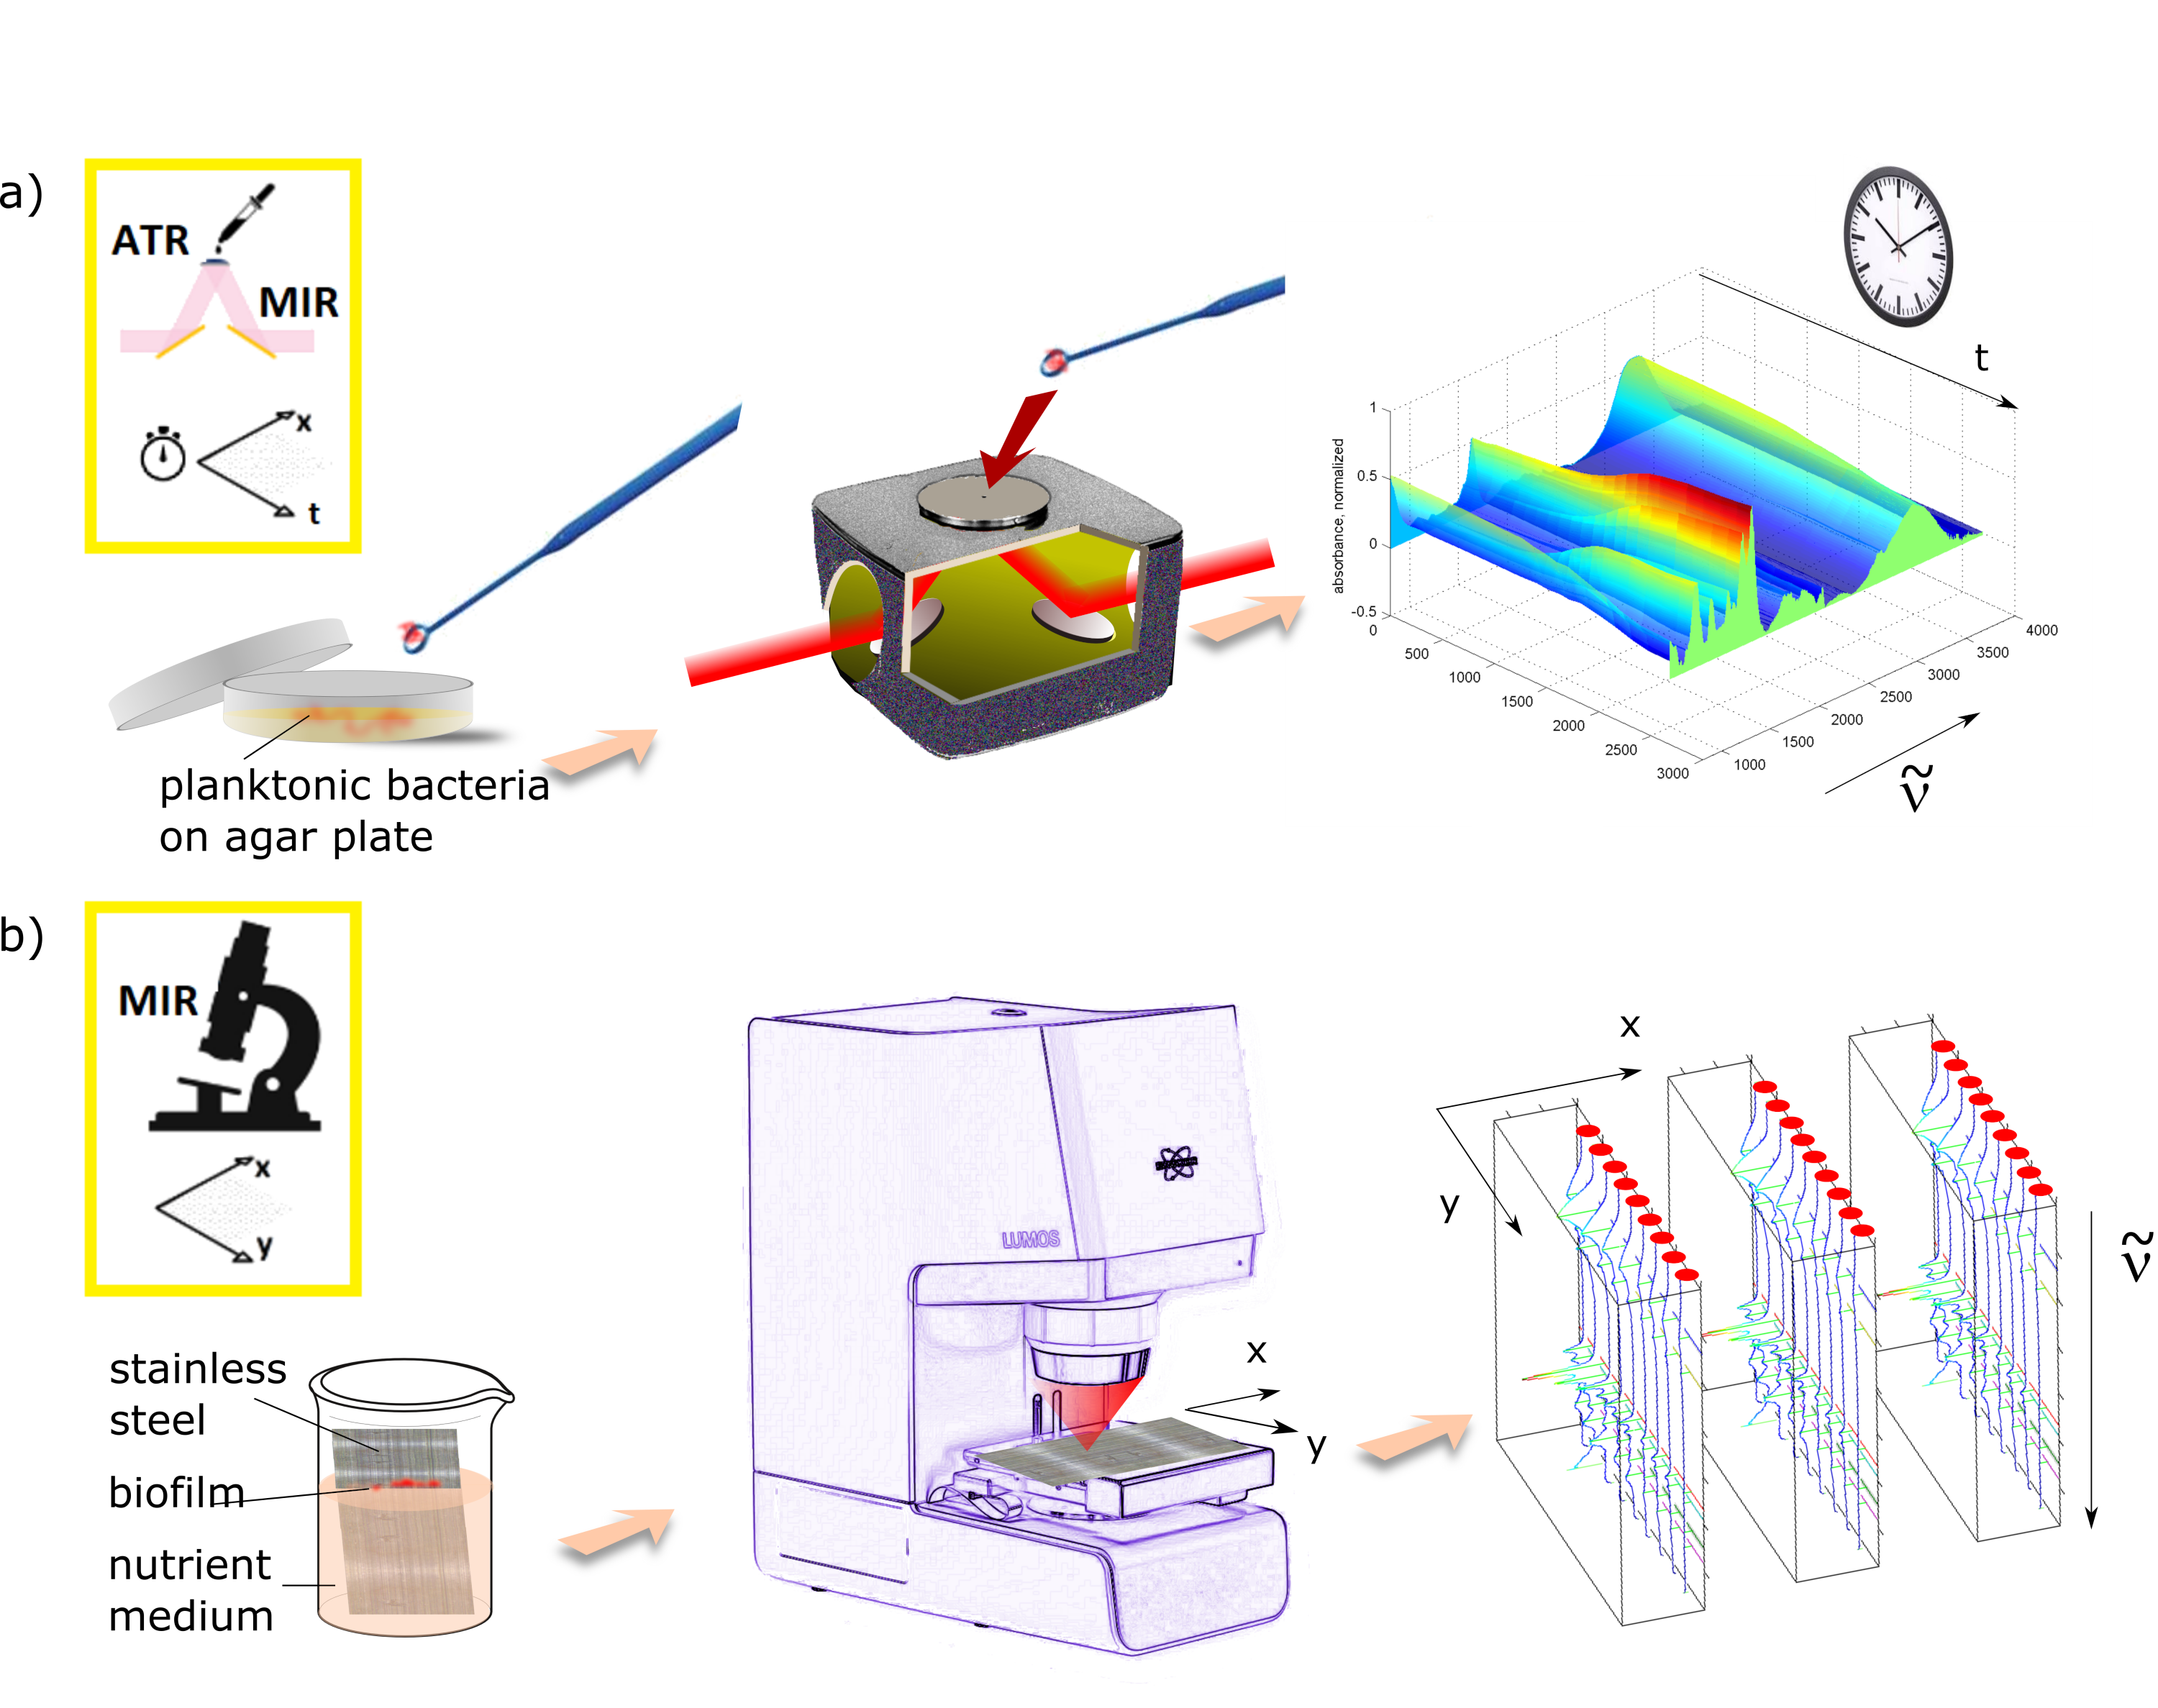
\includegraphics[width=1\columnwidth]{figures/figure1_compressed.png}};
\begin{scope}[x={(image.south east)},y={(image.north west)}]
% \node at (0.5,0.5) { \includegraphics[width=1\columnwidth]{figures/figure1.png}};
    %% HERE WILL BE SOME NOTATIONS/ETC (I USE THE COORDINATE SYSTEM TO DRAW THEM ON TOP OF THE IMAGE)
    %% AND GRID that are commented
    %   \draw[help lines,xstep=.1,ystep=.1] (0,0) grid (1,1);
    %   \draw[help lines,xstep=.05,ystep=.05] (0,0) grid (1,1);
    %   \foreach \x in {0,1,...,9} { \node [anchor=north] at (\x/10,0) {0.\x}; }
    %   \foreach \y in {0,1,...,9} { \node [anchor=east] at (0,\y/10) {0.\y};}
 \end{scope}
\end{tikzpicture}
  \caption{FTIR techniques and the sample preparation: (a) Petri dish with planktonic bacteria on agar; biomass is taken with a loop and put onto the ATR. Only the ATR part of the much larger FTIR spectrometer is shown.  The MIR spectrum of the drying biomass is watched over time; (b) The stainless steel plate with biofilm is taken from the nutrient medium, put under the FTIR microscope and raster scanned. Each raster point sketched as red dots, corresponds to a spectrum.}
 \label{fig:FTIRtechniques}
\end{figure}



\subsection{Data post-processing procedures}

\mynote{what is corrected for background?}
All spectra were corrected for the background. Additionally, Standard Normal Variate (SNV) Normalization was applied on the 2D scan spectra to account for intensity variations that usually occur at reflection measurements of uneven surfaces. For comparison between data from reflection measurements and ATR  measurements, systematic differences due to transmission through the ATR crystal and different penetration depth into the sample have to be taken into account. Each 2D raster-scan yielded a stack of spectra. In Fig 2D Scan b), such a typical stack is shown. The most prominent representatives of the respective molecular vibration are marked by vertical lines, such as lipids, proteins and poly saccharides.

For a sample which is highly specular like a glassy or crystalline substance as well as for biomass with high density [9] , the signal measured by transflexion is dominated by the specular reflectance R at the sample surface. As shown in Figure 4, two main trends are significant that indicate dominating reflection: the shift of peaks around 1500 cm-1 towards higher wavenumbers, and the flattening of the broad peak in the OH-region around 3700 cm-1.




%%%%%%%%%%%%%%%%%%%%%%%%%%%%%%%%%%%%%%%%%%
\section{Results}


\subsection{Specific spectra of strains}

The three strains primarily showed differences in the Polysaccharide region, which is in good accordance with other biofilm measurements \cite{Mosharaf_BioWaste_2018} .

\subsection{Time-resolved monitoring and analysis of bacteria aging due to drying}


\begin{figure}[ht]
\begin{tikzpicture}
\node[anchor=south west, inner sep=0] (image) at (0,0) {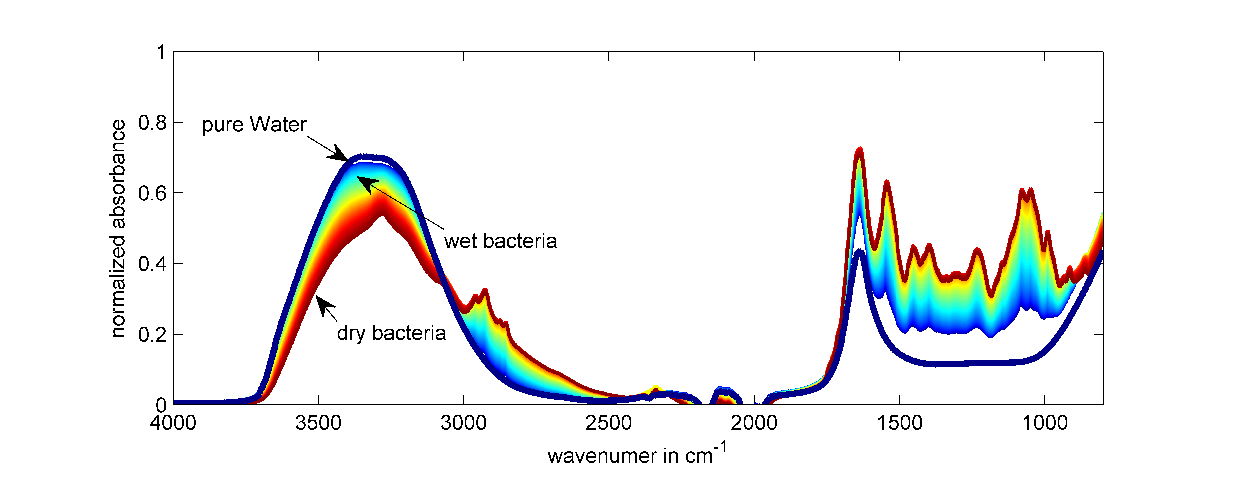
\includegraphics[width=1\columnwidth]{figures/pseudoBac_2_drying_water_2.eps}};
\begin{scope}[x={(image.south east)},y={(image.north west)}]
 \end{scope}
\end{tikzpicture}
  \caption{Drying process of adherent \textit{P. fragii }observed by FTIR ATR spectroscopic measurement. For comparison the spectrum of pure water (dark blue) is added. }
 \label{fig:dryPureWater}
\end{figure}
According to the observation of the drying process of  \textit{P. fragii } in figure \ref{fig:dryPureWater}, the absorbance of water dominates the spectral O-H regions of 4000-2500 cm$^{-1}$ as well as the Amide regions at 1800 to 1700 cm$^{-1}$. These regions can hardly be analyzed regarding bacteria in a humid state. During drying, the O-H regions absorb less, while the absorbance at 3000 cm$^{-1}$ and lower wavenumbers increases. 


\begin{figure}[ht]
\begin{tikzpicture}
\node[anchor=south west, inner sep=0] (image) at (0,0) {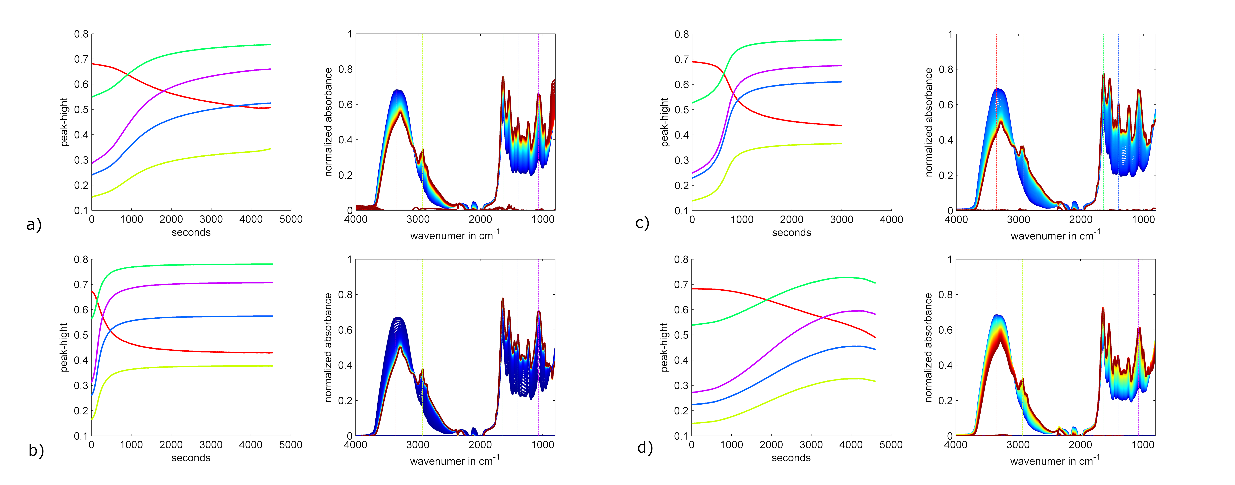
\includegraphics[width=1\columnwidth]{figures/all_drying.eps}};
\begin{scope}[x={(image.south east)},y={(image.north west)}]
 \end{scope}
\end{tikzpicture}
  \caption{Drying process of adherent \textit{P. fragii }(a,b), \textit{Brochotrix} (c) and \textit{Steno} (d) observed by FTIR ATR spectroscopic measurement. The height of selected peaks, plotted over time, show exponential behavior. The color of the plotted lines corresponds to the colors of the vertical peak position cursors in the spectrum.}
 \label{fig:dryingprocess}
\end{figure}




\begin{figure}[ht]
\begin{tikzpicture}
\node[anchor=south west, inner sep=0] (image) at (0,0) {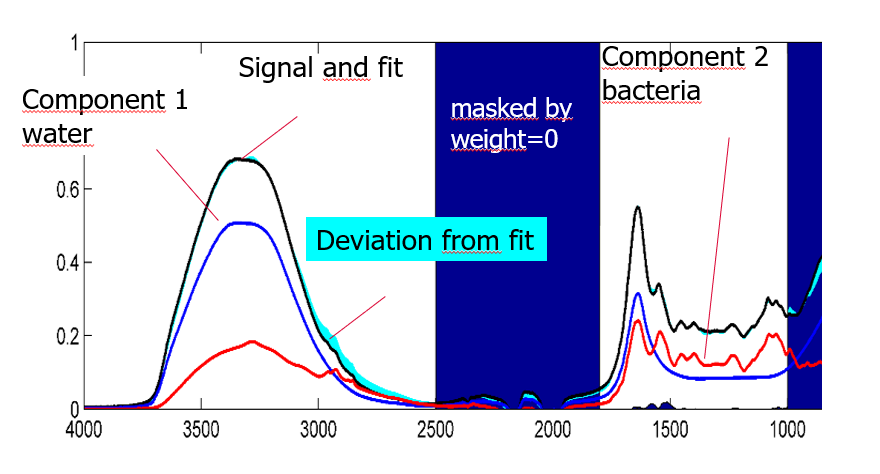
\includegraphics[width=1\columnwidth]{figures/Fitting.png}};
\begin{scope}[x={(image.south east)},y={(image.north west)}]
 \end{scope}
\end{tikzpicture}
  \caption{Decomposition of of adherent  \textit{Brochotrix} .}
 \label{fig:fitting}
\end{figure}
Figure 1 (exponential behavior, spectra changes over time and corresponding peak heights [pls. correct misprint]) – an easy-to-understand figure, goes first; Figure 2 and Figure 3 (decomposition of wet biofilms (or planktonic?) with this fit procedure (has to be described in postprocessing section, has be to described in the captions: what do we see here (non-valid region?)? no axes given.

Figures 3  a) and b) show the same drying process on a different time scale, a) the startof the drying process, and b) the long term behavior. While P. fragii (a,b), Brochotrix (c) could be easily dried and resulted in stable spectrum of the dry sample,  the Steno d) started to agglomerate and crumble.  
\subsection{}


% % Example of a figure that spans the whole page width (the commands \widefigure and \begin{paracol}{2}, \linenumbers, and\switchcolumn need to be present). The same concept works for tables, too.
% \end{paracol}
% \begin{figure}[h]	
% \widefigure
% 
\includegraphics[width=15 cm]{Definitions/logo-mdpi}
% \caption{This is a wide figure.\label{fig2}}
% \end{figure}  

% \begin{paracol}{2}
% \linenumbers
% \switchcolumn


\subsection{Analysis of spatial distribution and chemical heterogeneity}
\mynote{
should go first as it is successful results (also to cite a paper showing that the spectra are correct)
\textbf{Figures have to be commented/corrected:
}
Figure 1 (biofilm on stainless steel was raster scanned (13x40 points is not clear); I guess there is quite an information to comment here (e.g. they like an air/water interface more).

Figure 2 Pseudomonas simiae of varying thickness

Here to discuss: different thicknesses results in the different magnitude of absorbance, at some point we observe abnormal behavior; there is also spatial information (e.g. Amide 2 vs P-O stretching vs C-H – there are some inhomogeneities, any idea about this?); 

Figure the vertical lines are not described in the caption, why? Is this figure corresponds to a figure with a hand (anaerobic region/air)? Can it be a cause of some inhomogeneous spatial distribution?}

\begin{figure}[ht]
\begin{tikzpicture}
\node[anchor=south west, inner sep=0] (image) at (0,0) {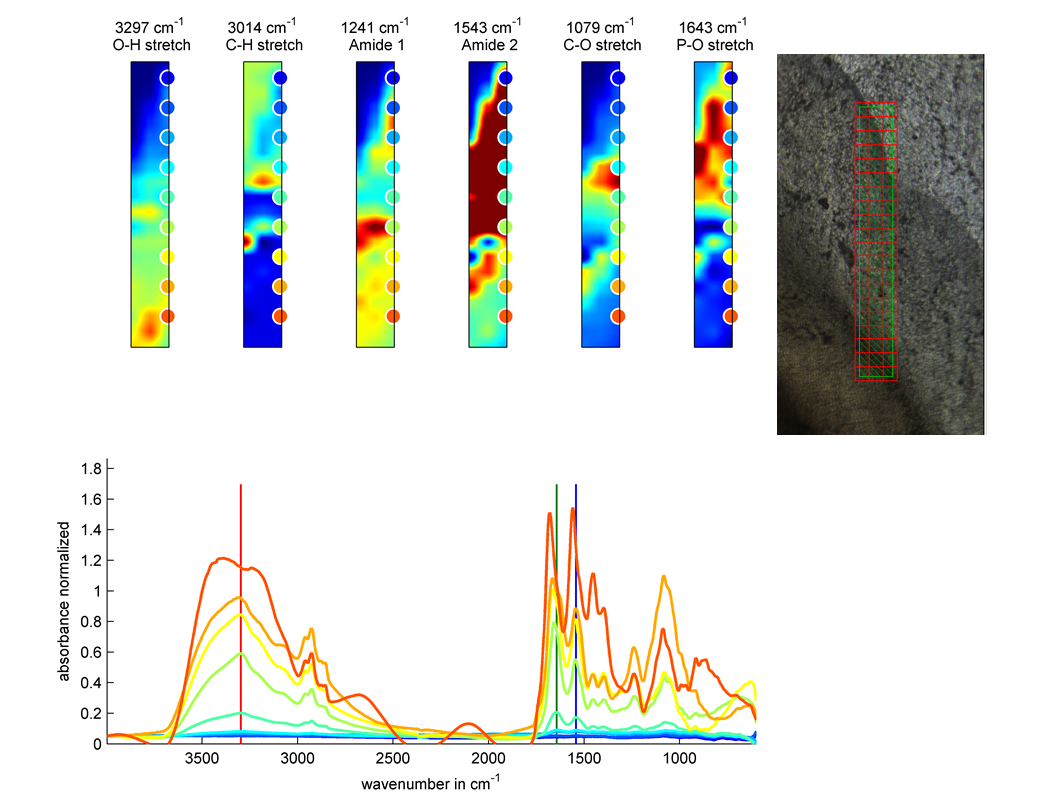
\includegraphics[width=1\columnwidth]{figures/spectra_of_dried_Pseudomonas_simiae_biofilm.png}};
\begin{scope}[x={(image.south east)},y={(image.north west)}]
% \node at (0.5,0.5) { \includegraphics[width=1\columnwidth]{figures/figure1.png}};
    %% HERE WILL BE SOME NOTATIONS/ETC (I USE THE COORDINATE SYSTEM TO DRAW THEM ON TOP OF THE IMAGE)
    %% AND GRID that are commented
    %   \draw[help lines,xstep=.1,ystep=.1] (0,0) grid (1,1);
    %   \draw[help lines,xstep=.05,ystep=.05] (0,0) grid (1,1);
    %   \foreach \x in {0,1,...,9} { \node [anchor=north] at (\x/10,0) {0.\x}; }
    %   \foreach \y in {0,1,...,9} { \node [anchor=east] at (0,\y/10) {0.\y};}
 \end{scope}
\end{tikzpicture}
  \caption{Spectra of dried Pseudomonas.}
 \label{fig:sp_dried_pseudomonas}
\end{figure}

\begin{figure}[ht]
\begin{tikzpicture}
\node[anchor=south west, inner sep=0] (image) at (0,0) {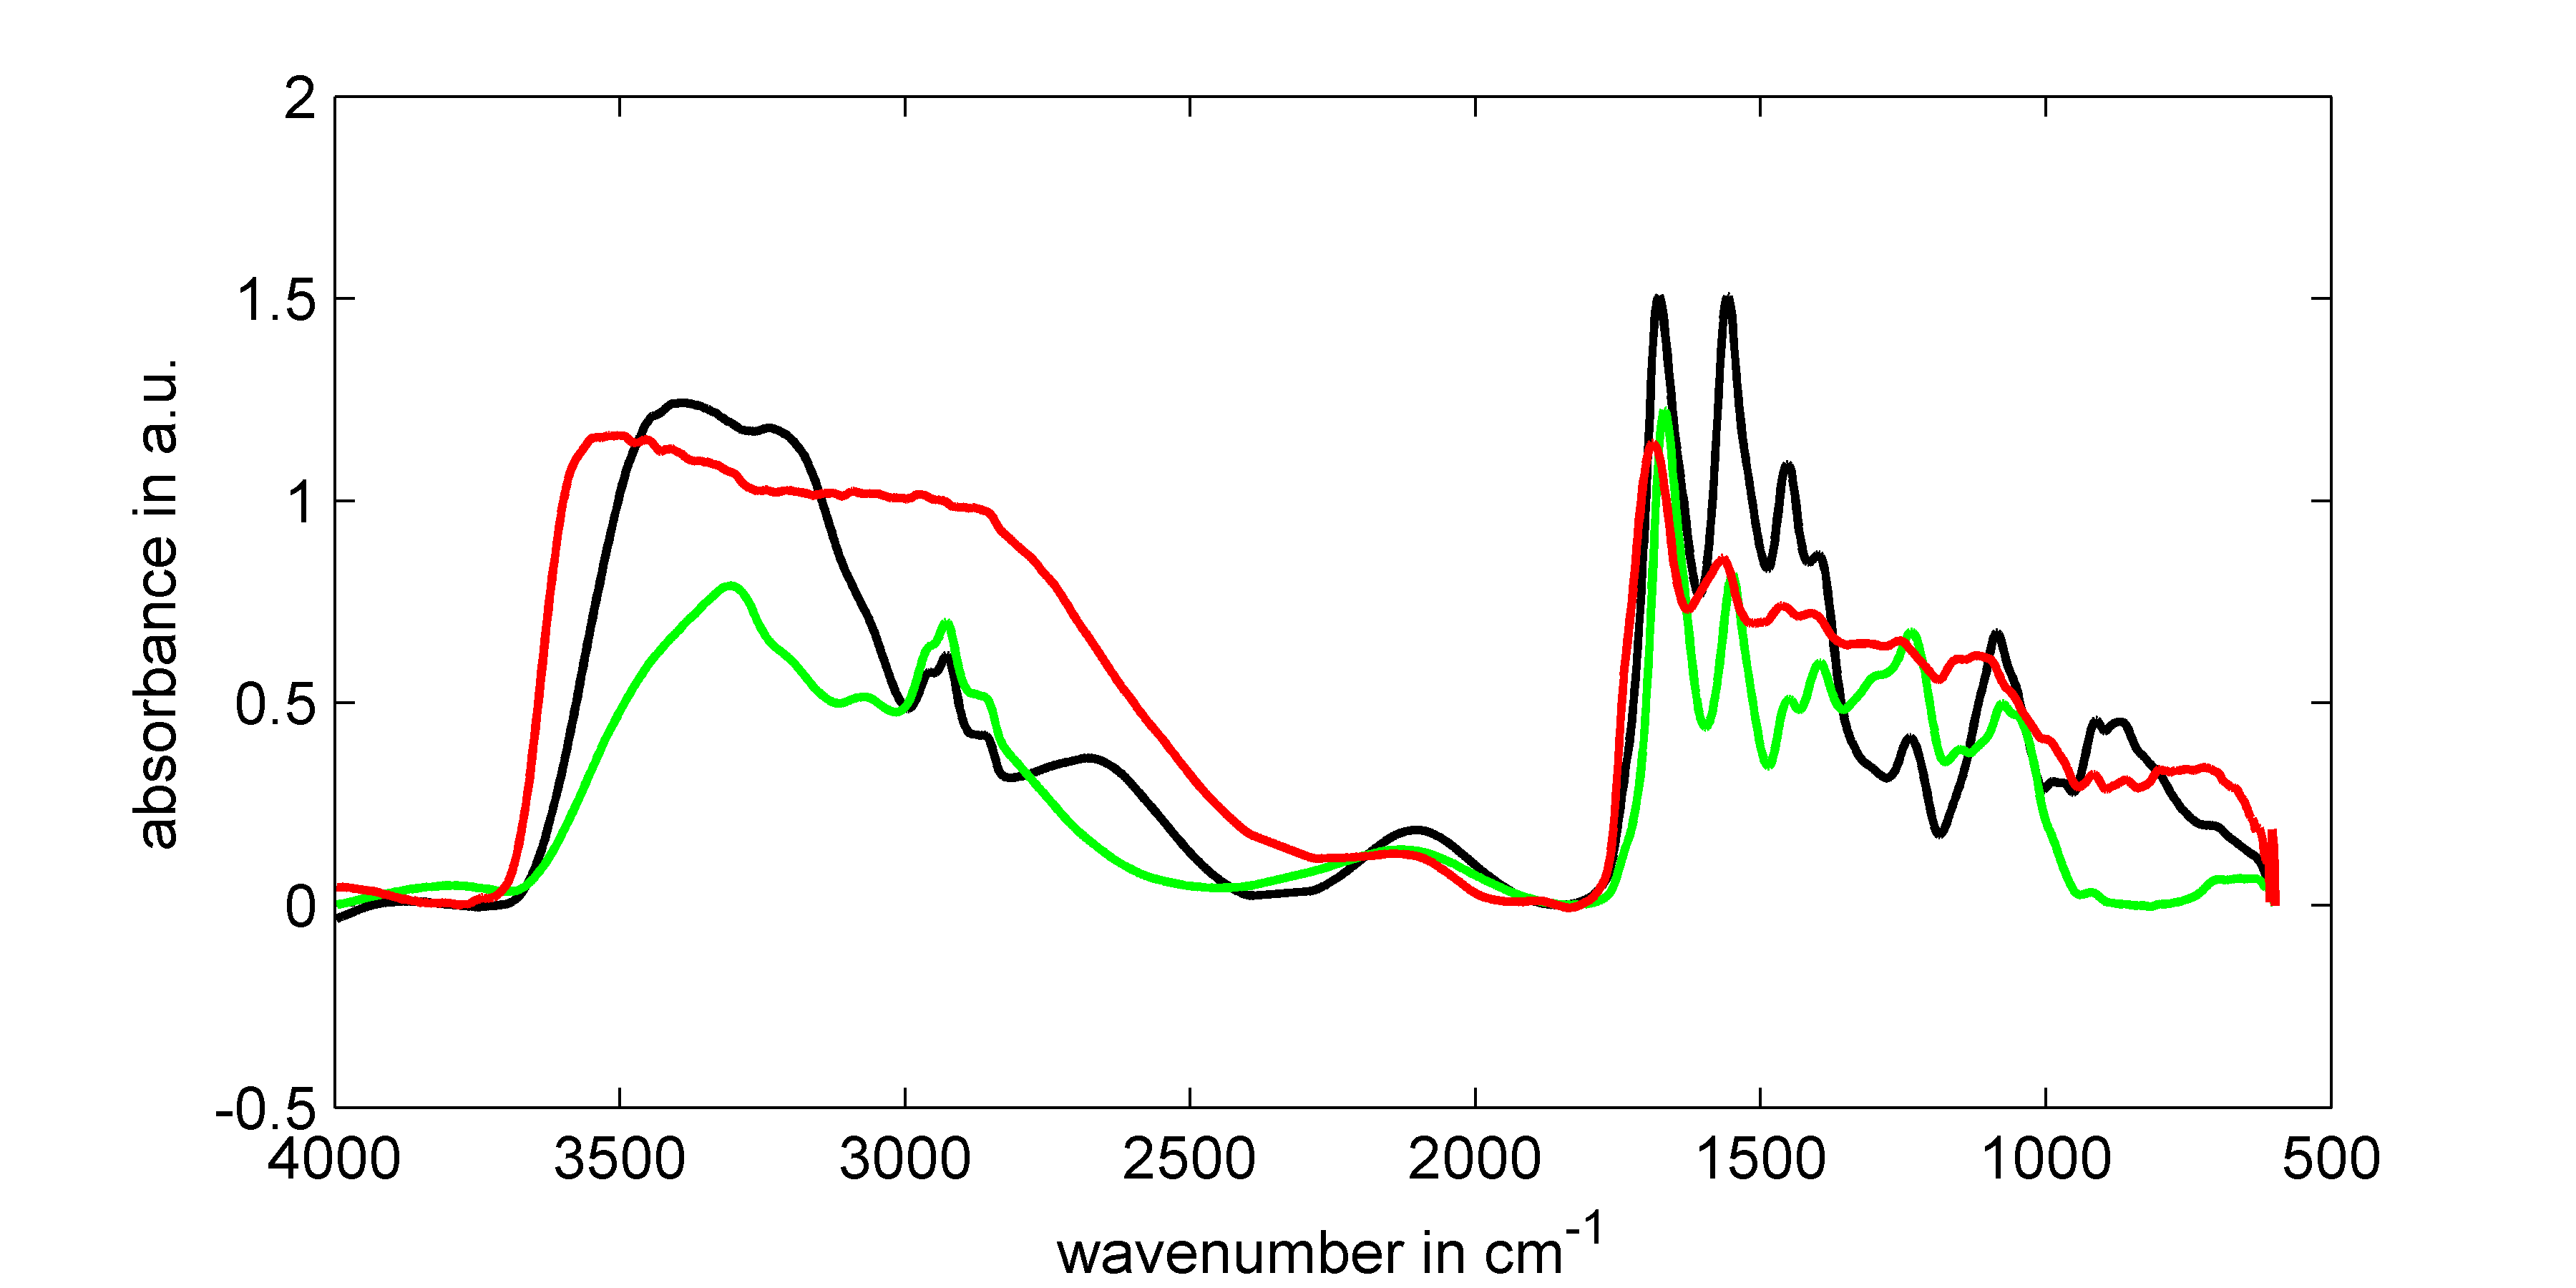
\includegraphics[width=1\columnwidth]{figures/fringes_tr_ref.png}};
\begin{scope}[x={(image.south east)},y={(image.north west)}]
% \node at (0.5,0.5) { \includegraphics[width=1\columnwidth]{figures/figure1.png}};
    %% HERE WILL BE SOME NOTATIONS/ETC (I USE THE COORDINATE SYSTEM TO DRAW THEM ON TOP OF THE IMAGE)
    %% AND GRID that are commented
    %   \draw[help lines,xstep=.1,ystep=.1] (0,0) grid (1,1);
    %   \draw[help lines,xstep=.05,ystep=.05] (0,0) grid (1,1);
    %   \foreach \x in {0,1,...,9} { \node [anchor=north] at (\x/10,0) {0.\x}; }
    %   \foreach \y in {0,1,...,9} { \node [anchor=east] at (0,\y/10) {0.\y};}
 \end{scope}
\end{tikzpicture}
  \caption{Artefacts in spectra of dried Pseudomonas.}
 
 \label{fig:sp_atrefacts}
\end{figure}
Permeability of the biofilm has been neglected, though biofilms do show a permeability different from zero \cite{Vogt_PermeabilityBiofilm_2013}, which would already slightly influence reflection and transmission at the air/biofilm interface. The permeabilty of steel 



%%%%%%%%%%%%%%%%%%%%%%%%%%%%%%%%%%%%%%%%%%
\section{Discussion}

Authors should discuss the results and how they can be interpreted from the perspective of previous studies and of the working hypotheses. The findings and their implications should be discussed in the broadest context possible. Future research directions may also be highlighted.


\cite{Mayrhoefer_script_2021} At the same time, we should better announce the index of refraction also as index of refraction function. However, the index of refraction function is not in the center of attention in this chapter, because it is, as we will see, only indirectly a material property. Mind: absorption icreases reflection. Chapter 3.3 Excursus: Dispersion relations and Beer’s law.
( ad transmission measurements)  Accordingly, for larger thickness, T reaches eventually zero and R is what remains. This causes a strong shift for stronger bands, since for the comparably weak oscillators in organic and biological materials, reflectance is mostly influenced  by dispersion and the maximum of the real part of the dielectric function is redshifted compared to 
the oscillator position. The superposition of R and T also leads to the phenomenon that 
intermediately a second band maximum appears. S. 135 Therefore, reflectance does not influence the band positions in transmittance for small thicknesses 
even for larger oscillator strength. .
However, the fluctuations of the band positions due to 
interferences still occur, regardless of how the baseline correction is carried out. 
( ad transflection measurements) S 136 4.3  .
Then, in 2012, seemingly strange variations of the  relative intensities of bands with layer thickness were found.amplitude of interference fringes only zero for perfect conductors
Conductivity of  Ag, Cu, Au and steel is 62, 58 44 and about 14$\times$10\textsuperscript{6} Siemens/m. Thus, R <1. 
Therefore, even for organic and biologic materials the deviations from Beer’s law are strong as can be seen in Fig. 4-7, left side, and the underlying interference fringes can be detected by the fact that in-between peaks the baseline does not reach zero and shows undulations.

We are dealing with materials with low oscillator strength,  organic or biologic materials. (corresponds with low area under peak) 
We only see \textit{apparent} absorbance. 
We can assume that in general the biofilm does not represent a perfect plane layer. Thus the reflected light is incoherent and interference will hardly occur. In addition, transflection measurements in the MIR region allow a higher sample density before the reflection at the sample surface becomes significantly high. Measurements in the NIR region are prone to interference and the corresponding fringes in the spectrum. Anyway, interference should be kept in mind. Therefore the spectrum in spectral regions with low absorption, i.e. between the characteristic absorption bands, should be checked regarding fringes, caused by interference.The measurement of wet biofilms is only possible in case of a high bacteria concentration as otherwise the spectrum is masked by the water spectrum. device with geblaese to dry spot of measurement Assumption: almost linear relation between density / refractive index and reflectivity. Hagens-Ruben equation , more true for higher wavelength --- towards 800 cm\textsuperscript{-1}.
Specular Spectral Reflectance Of ALS1304 Stainless Steel At Near-Normal Incidence

However, the index of refraction function is not in the center of 
attention in this chapter, because it is, as we will see, only indirectly a material property. 
Unfortunately, this also means automatically that the index of absorption function as its imaginary 
part is neither a material property. Therefore, it also does not automatically make sense to try to 
analyze an absorbance spectrum by a band fit, but we will see that there are important exceptions. 

S 155
Again, I highly recommend the book of Pocchi Yeh\textit{} , which I have 
used for large parts of this chapter as basis and inspiration.22 In addition, Born and Wolf’s “Principles 
of Optics, is an excellent read3 and also, Hecht’s Optics.21 To understand phenomena related to 
total internal reflection I recommend Internal Reflection and ATR Spectroscopy
27 by M. Milosevic, 

proteins changed from a helical conformation (bands between 1660 cm\textsuperscript{-1} and 1650 cm\textsuperscript{-1} at a lower pH to an unordered random coil (band between 1650 cm\textsuperscript{-1}
and 1640 cm\textsuperscript{-1}  at a higher pH.7,22 In addition, the intensities of peaks at 1654 cm\textsuperscript{-1}(C=O), 1529 cm\textsuperscript{-1} and 1234-1250 cm\textsuperscript{-1}  considerably decreased with the increasing pH, arising from the destruction of amide groups in proteins \cite{Wang_pH_EPS:_2012}


%%%%%%%%%%%%%%%%%%%%%%%%%%%%%%%%%%%%%%%%%%
\section{Conclusions}

This section is not mandatory, but can be added to the manuscript if the discussion is unusually long or complex.

%%%%%%%%%%%%%%%%%%%%%%%%%%%%%%%%%%%%%%%%%%
% \section{Patents}

% This section is not mandatory, but may be added if there are patents resulting from the work reported in this manuscript.

%%%%%%%%%%%%%%%%%%%%%%%%%%%%%%%%%%%%%%%%%%
\vspace{6pt} 

%%%%%%%%%%%%%%%%%%%%%%%%%%%%%%%%%%%%%%%%%%
%% optional
%\supplementary{The following are available online at \linksupplementary{s1}, Figure S1: title, Table S1: title, Video S1: title.}

% Only for the journal Methods and Protocols:
% If you wish to submit a video article, please do so with any other supplementary material.
% \supplementary{The following are available at \linksupplementary{s1}, Figure S1: title, Table S1: title, Video S1: title. A supporting video article is available at doi: link.} 

%%%%%%%%%%%%%%%%%%%%%%%%%%%%%%%%%%%%%%%%%%
\authorcontributions{Conceptualization, X.X. and Y.Y.; methodology, X.X.; software, X.X.; validation, X.X., Y.Y. and Z.Z.; formal analysis, X.X.; investigation, X.X.; resources, X.X.; data curation, X.X.; writing---original draft preparation, X.X.; writing---review and editing, X.X.; visualization, X.X.; supervision, X.X.; project administration, X.X.; funding acquisition, Y.Y. All authors have read and agreed to the published version of the manuscript.}

\funding{This research was funded by NAME OF FUNDER grant number XXX.}


\dataavailability{The data presented in this study are available on request from the corresponding author. The data are not publicly available due to legal reasons.} 

\acknowledgments{XXX}

\conflictsofinterest{The authors declare no conflict of interest.} 

%% Optional
% \sampleavailability{Samples of the compounds ... are available from the authors.}

%%%%%%%%%%%%%%%%%%%%%%%%%%%%%%%%%%%%%%%%%%
%% Only for journal Encyclopedia
%\entrylink{The Link to this entry published on the encyclopedia platform.}

%%%%%%%%%%%%%%%%%%%%%%%%%%%%%%%%%%%%%%%%%%
%% Optional
\abbreviations{The following abbreviations are used in this manuscript:\\

\noindent 
\begin{tabular}{@{}ll}
FTIR & Fourier-transform infrared spectroscopy\\
ATR & Attenuated total reflection\\
MIR & Mid-infrared\\
LD & Linear dichroism
\end{tabular}}

%%%%%%%%%%%%%%%%%%%%%%%%%%%%%%%%%%%%%%%%%%
\end{paracol}
\reftitle{References}

% Please provide either the correct journal abbreviation (e.g. according to the “List of Title Word Abbreviations” http://www.issn.org/services/online-services/access-to-the-ltwa/) or the full name of the journal.
% Citations and References in Supplementary files are permitted provided that they also appear in the reference list here. 

%=====================================
% References, variant A: external bibliography
%=====================================
\externalbibliography{yes}
\bibliography{bibliography.bib}

% %=====================================
% % References, variant B: internal bibliography
% %=====================================
% \begin{thebibliography}{999}
% % Reference 1
% \bibitem[Author1(year)]{ref-journal}
% Author~1, T. The title of the cited article. {\em Journal Abbreviation} {\bf 2008}, {\em 10}, 142--149.
% % Reference 2
% \bibitem[Author2(year)]{ref-book1}
% Author~2, L. The title of the cited contribution. In {\em The Book Title}; Editor1, F., Editor2, A., Eds.; Publishing House: City, Country, 2007; pp. 32--58.
% % Reference 3
% \bibitem[Author3(year)]{ref-book2}
% Author 1, A.; Author 2, B. \textit{Book Title}, 3rd ed.; Publisher: Publisher Location, Country, 2008; pp. 154--196.
% % Reference 4
% \bibitem[Author4(year)]{ref-unpublish}
% Author 1, A.B.; Author 2, C. Title of Unpublished Work. \textit{Abbreviated Journal Name} stage of publication (under review; accepted; in~press).
% % Reference 5
% \bibitem[Author5(year)]{ref-communication}
% Author 1, A.B. (University, City, State, Country); Author 2, C. (Institute, City, State, Country). Personal communication, 2012.
% % Reference 6
% \bibitem[Author6(year)]{ref-proceeding}
% Author 1, A.B.; Author 2, C.D.; Author 3, E.F. Title of Presentation. In Title of the Collected Work (if available), Proceedings of the Name of the Conference, Location of Conference, Country, Date of Conference; Editor 1, Editor 2, Eds. (if available); Publisher: City, Country, Year (if available); Abstract Number (optional), Pagination (optional).
% % Reference 7
% \bibitem[Author7(year)]{ref-thesis}
% Author 1, A.B. Title of Thesis. Level of Thesis, Degree-Granting University, Location of University, Date of Completion.
% % Reference 8
% \bibitem[Author8(year)]{ref-url}
% Title of Site. Available online: URL (accessed on Day Month Year).
% \end{thebibliography}

% If authors have biography, please use the format below
%\section*{Short Biography of Authors}
%\bio
%{\raisebox{-0.35cm}{\includegraphics[width=3.5cm,height=5.3cm,clip,keepaspectratio]{Definitions/author1.pdf}}}
%{\textbf{Firstname Lastname} Biography of first author}
%
%\bio
%{\raisebox{-0.35cm}{\includegraphics[width=3.5cm,height=5.3cm,clip,keepaspectratio]{Definitions/author2.jpg}}}
%{\textbf{Firstname Lastname} Biography of second author}

% The following MDPI journals use author-date citation: Arts, Econometrics, Economies, Genealogy, Humanities, IJFS, JRFM, Laws, Religions, Risks, Social Sciences. For those journals, please follow the formatting guidelines on http://www.mdpi.com/authors/references
% To cite two works by the same author: \citeauthor{ref-journal-1a} (\citeyear{ref-journal-1a}, \citeyear{ref-journal-1b}). This produces: Whittaker (1967, 1975)
% To cite two works by the same author with specific pages: \citeauthor{ref-journal-3a} (\citeyear{ref-journal-3a}, p. 328; \citeyear{ref-journal-3b}, p.475). This produces: Wong (1999, p. 328; 2000, p. 475)

%%%%%%%%%%%%%%%%%%%%%%%%%%%%%%%%%%%%%%%%%%
%% for journal Sci
%\reviewreports{\\
%Reviewer 1 comments and authors’ response\\
%Reviewer 2 comments and authors’ response\\
%Reviewer 3 comments and authors’ response
%}
%%%%%%%%%%%%%%%%%%%%%%%%%%%%%%%%%%%%%%%%%%
\end{document}

